%!TEX root = ..\..\main.tex
\chapter{Introduction}
\label{Ch:CouplingIntro}

\lhead{Chapter \ref{Ch:CouplingIntro}. \emph{Introduction}} % This is for the header on each page


\section{The Ising model}
\label{sec:Ising}
	The Ising model is named after Ernst Ising who studied it in his 1924 thesis \cite{Ising1925-nd} under the supervision of Wilhelm Lenz, who introduced the model in \cite{Lenz1920-bn}. It was originally motivated by the phenomenon of ferromagnetism but it has since found application to apply to numerous other situations in both physics and other fields \footnote{See \cite[notes of Section 1.4.2]{Friedli2017-xm} for a list of references concerning this.}.

	The Ising model occupies a prominent position in the statistical physics literature. This is largely due to the existence of a phase transition; a sharp transition in the large scale behaviour of the model as a parameter crosses a critical value. The transition was first shown to exist by Rudolph Peierls \cite{Peierls1936-pu} in what was the first proof of the existence of a phase transition for any model with purely local interactions in statistical mechanics.
	Additionally, the Ising model is both relatively simple, and also mathematically tractable in some non-trivial cases \cite{Onsager1944-li}. These qualities are rare among models with a phase transition and so the Ising model has become somewhat of a staple for both studying phase transitions and testing new statistical mechanics techniques.

	The model is a probability distribution on spin configurations - assignments of $+1$ and $-1$ spins to each vertex in a finite graph $G = (V, E)$. The set of all possible configurations is
	\begin{equation}
		\Omega = \{-1, +1\}^V
	\end{equation}
	and for a particular configuration, $\sigma \in \Omega$, we refer to the spin of a particular vertex $i \in V$ as $\sigma[i]$. Each configuration has an associated energy, given by 
	\begin{equation}
		H_{G, \beta, h}(\sigma) = -\beta \sum_{ij \in E} \sigma[i] \sigma[j] - h\sum_{i \in V} \sigma[i]
	\end{equation}
	where $\beta \in [0, \infty)$ is the inverse temperature, and $h \in \mathbb{R}$ is the magnetic field. 

	The Gibbs measure is the distribution on $\Omega$ that characterises the Ising model and it is defined by
	\begin{equation}
		\pi_{G, \beta, h}(\sigma) \propto \exp(-H_{G, \beta, h}(\sigma)).
		\label{eq:gibbsmeasurefull}
	\end{equation}
	In everything that follows, we will be concerned only with the zero-field ($h = 0$) Ising model. This gives us the slightly simpler form for the Gibbs measure,
	\begin{equation}
		\pi_{G, \beta}(\sigma) \propto \exp \left( \beta \sum_{ij \in E} \sigma[i] \sigma[j] \right), \qquad \sigma \in \{-1, 1\}^V.
		\label{eq:gibbsmeasure}
	\end{equation}

	\subsection{The phase transition}
	\label{sec:the phase transition}
	An in depth study of the Ising phase transition and its associated critical temperature will not be needed for this work. However, we will still wish to refer to it occasionally and so here we give a workable description of the phase transition on lattices.

	Consider the Gibbs measure with zero-field \eqref{eq:gibbsmeasure} in the limits $\beta \downarrow 0$ and $\beta \uparrow \infty$. It is easy to see that in the former limit, the measure is uniform across all configurations and in the latter limit, the measure assigns all weight to the constant configurations $\sigma^- = (-1, -1, \dots, -1)$ and $\sigma^+ = (+1, +1, \dots, +1)$. This leads to the following overly simplistic description of the phase transition. It is an abrupt change in distribution that occurs as we increase the temperature; from distributions concentrated on states whose spins mostly agree, to distributions producing states which have roughly equal numbers of plus and minus spins.

	To be slightly more concrete we define quantities called the magnetization and magnetization density. The \emph{magnetization} on a volume $\Lambda \subseteq V$ is defined as 
	\begin{equation}
		M_\Lambda(\sigma) = \sum_{i \in \Lambda} \sigma[i].
	\end{equation}
	Normalizing this gives the \emph{magnetization density}, $M_\Lambda(\sigma)/|\Lambda|$. On the $d$-dimensional torus with side length $L$, $G(L) = (\mathbb{Z}/L\mathbb{Z})^d$, the quantity
	\begin{equation}
		m(\beta) = \lim_{L \rightarrow \infty} \expect_\beta \left|\frac{M_{G(L)}(\sigma)}{|G(L)|} \right|
		\label{eq:limitmagnetizationdensity}
	\end{equation}
	depends on the inverse temperature $\beta$. When $d = 1$, $m(\beta) = 0$ for any $\beta$ and there is no phase transition. However, when $d > 1$, there exists some critical $\beta_c(d)$ such that $m(\beta) = 0$ for $\beta < \beta_c(d)$ and $m(\beta) > 0$ for $\beta > \beta_c(d)$ \cite{Friedli2017-xm}. This $\beta_c(d)$ is the critical inverse temperature at which we observe a phase transition.

	% On most graphs [FIND OUT WHICH] the Ising model undergoes a phase transition at a critical inverse temperature $\beta_c = \beta_c(G)$ that is dependent on the graph. Roughly speaking, for $\beta < \beta_c$ (the high-temperature regime), the correlation of spins dies off quickly with the distance between them and for $\beta > \beta_c$ (the low-temperature regime), spins remain correlated at a large distance.

	% [EXTEND]

\section{Coupling from the past}
	One of the central challenges regarding the Ising model is how to efficiently sample from the Gibbs measure. Calculating the normalizing constant for \eqref{eq:gibbsmeasure}, known as the partition function, is a \#P-complete problem \cite{Jerrum1993-ii}. As such a direct approach to sampling is expected to be computationally intractable in general, and so other methods must be employed instead. One such method is Markov Chain Monte Carlo (MCMC). This involves constructing a Markov chain whose states are elements of $\Omega$ and whose stationary distribution is given by \eqref{eq:gibbsmeasure}. One can then obtain a sample by running this Markov chain for long enough that the output has distribution sufficiently close to \eqref{eq:gibbsmeasure}.
	% The zero-field ferromagnetic Ising model on finite graph $G = (V, E)$ at 
	% inverse temperature $\beta \geq 0$ has Gibbs measure
	%
	One difficulty in using MCMC is that one does not know a priori what constitutes "long enough". In principal, bounds on this time can be obtained, but in practise, proving these bounds can be very challenging.

	An alternative to classical MCMC called Coupling from the Past (CFTP) was introduced by Propp and Wilson \cite{Propp1996-cf}. Unlike MCMC, CFTP not only has an automatically determined running time, but it has the additional advantage of outputting exact samples from the stationary distribution. This does not come without a cost - CFTP has a random running time. Therefore, a key question towards evaluating the effectiveness of CFTP is understanding the distribution of its running time, that is, the \emph{coupling time}.

	In Chapters \ref{Ch:1D} and \ref{Ch:GeneralResults}, we will investigate the coupling time for the Ising heat-bath Glauber dynamics, both on the cycle, at any temperature, in Chapter \ref{Ch:1D}, and on any vertex transitive graph, at sufficiently high temperatures, in Chapter \ref{Ch:GeneralResults}. Our main result in each chapter will be proving that, when appropriately scaled, the distribution of the coupling time essentially converges to a Gumbel as the size of the graph increases. 

	\subsection{Ising heat-bath Glauber dynamics}
	\label{sec:heat-bath glauber dynamics definition}
	The continuous-time heat-bath Glauber dynamics for the Ising model is a Markov chain whose states are elements of $\Omega$ and whose stationary distribution is given by \eqref{eq:gibbsmeasure}. For a given graph $G = (V, E)$, and a given inverse temperature, $\beta$, we can describe the dynamics as follows. 

	Initialize every vertex in $V$ with a spin (for example, we could start in the all-plus configuration). To each vertex in $V$ we give an independent rate-one Poisson clock. For $\sigma \in \Omega$ and $i \in V$, define the probability 
	\begin{equation}
		p_i(\sigma) = \frac{\euler^{\beta S_i(\sigma)}}{\euler^{\beta S_i(\sigma)} + \euler^{-\beta S_i(\sigma)}}
		\label{eq:define p_i}
	\end{equation}
	where
	\begin{equation}
		S_i(\sigma) = \sum_{j \sim i} \sigma[j]
	\end{equation}
	is the sum of the spins of the neighbours of $i$, and $j \sim i$ denotes that $j$ is connected to $i$ with some edge $ij \in E$. Let $\sigma_t$ denote the spin configuration at time $t$. When the clock of vertex $i$ rings at some time $t$, we update $\sigma_t[i]$ to $+1$ with probability $p_i(\sigma_t)$, and to $-1$ otherwise.

	The probability $p_i(\sigma)$ is constructed so that it gives the probability that vertex $i$ is $+1$ if we sample it from $\pi$ \eqref{eq:gibbsmeasure} conditioned on every other vertex having its spin fixed by $\sigma$. Note that this causes the dynamics to have $\pi$ as its stationary distribution.

	\subsection{The coupling time}
	\label{sec:the coupling time}
	[THIS NEEDS A BIT OF REWRITING. DEFINE BOTH DISCRETE AND CONTINUOUS RMR. TALK ABOUT BOTH WAYS OF DOING THIS. GENERATE $V_K$ SEQUENCE VIA POISSON CLOCKS. START WITH DISCRETE, THEN USUAL, THEN N CLOCKS.]

	We now describe the two coupled chains from which we define the coupling time of the Ising heat-bath Glauber dynamics. It will prove convenient to first describe the discrete time chains along with their coupling and then discuss how to extend this coupling to the continuous time chain.	In order to define the discrete time coupling, we introduce a random mapping representation.

	Define $f: \Omega \times V \times [0,1] \mapsto \Omega$ via $f(\sigma, i, u) = \sigma'$ where $\sigma'[j] = \sigma[j]$ for $j \neq i$ and
	\begin{equation}
		\sigma'[i] = 
			\begin{cases}
				1, &u \leq p_i(\sigma),\\
				-1, &u > p_i(\sigma).
			\end{cases}
		\label{eq:plusorminusrules}
	\end{equation}

	We note that $f$ is monotonic, in the following sense. We define a partial ordering on $\Omega$ by writing that $\sigma \preceq \omega$ if $\sigma, \omega \in \Omega$ are such that $\sigma[i] \leq \omega[i]$ for all $i \in V$ (and similarly for $\sigma \succeq \omega$). Then for any fixed $i \in V$ and $u \in [0,1]$, if $\sigma \preceq \omega$ then $f(\sigma, i, u) \preceq f(\omega, i, u)$.
	
	Let $(\mathscr{V}_k, U_k)_{k \geq 1}$ be an i.i.d. sequence of copies of $(\mathscr{V}, U)$. Define top and bottom discrete time chains, $(\mathscr{T}_t)_{t\in \mathbb{N}}^\mathrm{DIS}$ and $(\mathscr{B}_t)_{t\in \mathbb{N}}^\mathrm{DIS}$, with initial states
	\begin{align}
		\mathscr{T}_0^\mathrm{DIS} &= (1, 1, \dots, 1)\\
		\mathscr{B}_0^\mathrm{DIS} &= (-1, -1, \dots, -1)
	\end{align}
	that update according to $\mathscr{T}_{t+1}^\mathrm{DIS} = f(\mathscr{T}_{t}^\mathrm{DIS}, \mathscr{V}_k, U_k)$ and $\mathscr{B}_{t+1}^\mathrm{DIS} = f(\mathscr{B}_{t}^\mathrm{DIS}, \mathscr{V}_k, U_k)$.

	We call the coupled process, $(\mathscr{B}_t^\mathrm{DIS}, \mathscr{F}_t^\mathrm{DIS})_{t\in \mathbb{N}}$, \emph{the discrete Ising heat-bath coupling}. From the monotonicity of $f$, $\mathscr{T}_t^\mathrm{DIS} \succeq \mathscr{B}_t^\mathrm{DIS}$, for all $t \geq 0$.

	There are two ways we can think about extending this process to our continuous-time chain. The first way is to "continuize it at rate n" [CITATION... I CAN'T FIND THIS IN LEVIN-PERES]. To do this we use the discrete process as defined above but the time between each update is an independent exponential with rate $n$. That is, the continuous-time top and bottom chains are defined as $(\mathscr{B}_t, \mathscr{T}_t) = (\mathscr{B}_{N_t}^\mathrm{DIS}, \mathscr{T}_{N_t}^\mathrm{DIS})$ where $N_t$ is an independent rate $n$ Poisson process. We call $(\mathscr{B}_t, \mathscr{T}_t)_{t\geq 0}$ simply, \emph{the Ising heat-bath coupling}.

	It is perhaps not immediately obvious that the continuous time top and bottom chains have the same dynamics we described in Section \ref{sec:heat-bath glauber dynamics definition}. This leads us to the second way of extending the discrete coupling to continuous time. Instead of updating the whole chain at rate $n$ and choosing a vertex to update on the $k$th update via $\mathcal{V}_k$, we can think of each vertex in the chain as having its own independent rate 1 Poisson clock that tells it when to update. To clarify, whenever the Poisson clock of any vertex $i$ rings at time $t$, we perform the $k$th update of the chain by setting $\mathcal{V}_k = i$ and updating as in the discrete case via $\mathscr{B}_t \leftarrow f(\mathscr{B}_t, \mathcal{V}_k, U_k)$ and $\mathscr{T}_t \leftarrow f(\mathscr{T}_t, \mathcal{V}_k, U_k)$.

	From the memoryless property of the exponential, the sequence $\mathcal{V}_1, \mathcal{V}_2, \dots$ that is generated is i.i.d.\ uniform on $V$. Since we have $n$ vertices updating at rate 1, the whole chain is updating at rate $n$, and so our two methods of extending the discrete coupling to continuous time are equivalent.

		
	

	


	% Let $\mathscr{V}$ and $U$ be independent, with $\mathscr{V}$ uniform on $V$ and $U$ uniform on $[0,1]$. Then, updating our chain at rate $n = |V|$, and performing updates from $\sigma$ to $\sigma'$ according to $\sigma' = f(\sigma, \mathscr{V}, U)$, we recover the dynamics described in Section \ref{sec:heat-bath glauber dynamics definition}.

	This leads to a more descriptive explanation of the continuous time coupling: the top and bottom chains share the same rate-one Poisson clocks at each vertex, and upon updating that vertex, we share the same uniform random variable $U$ between the two chains to determine whether to update to a plus or minus according to \eqref{eq:plusorminusrules}.

	The \emph{coupling time} of the Ising heat-bath process is the random variable
	\begin{equation}
		T = \inf \left\{t : \mathscr{T}_t = \mathscr{B}_t \right\}.	
	\end{equation}
	This is the main object of interest for our analysis. Note that the coupling time is not just a property of the Ising heat-bath process, but also of the coupling we have chosen. In Section \ref{sec:information percolation on the cycle} we will make a change to the coupling we use to make the analysis easier. Some care will need to be taken to verify that the coupling time is not affected by this change.

	\subsection{Equivalence of discrete and continuous coupling time}
	So far we have stated that the running time of CFTP has the same distribution as the coupling time. In fact, we have glossed over one important detail. Namely, CFTP is exclusively run in discrete time, and our coupling time is defined by the continuous time dynamics. Therefore, for our motivation to be reasonable, we would like to show some sort of equivalence between the distributions of the discrete and continuous coupling times. We do this via Proposition \ref{claim:discrete vs continuous distributions}. 

	\begin{proposition}
	\label{claim:discrete vs continuous distributions}
		Let $(N_n)_{n \in \mathbb{N}}$ be a sequence of positive integer-valued random variables, and $(m_n)_{n \in \mathbb{N}}$ be a non-decreasing sequence of integers such that $N_n \geq m_n$ for all $n$ and $\lim_{n \rightarrow \infty} m_n = \infty$. Let $T(n)$ be the random time it takes for a rate $\lambda$ Poisson clock to go off $n$ times. That is, $T(n) \sim \mathrm{Erlang}(n, \lambda)$.

		Let $a_n$ and $b_n$ be positive deterministic sequences such that $b_n / a_n \rightarrow \infty$ and
		\begin{equation}
			\frac{b_n^2}{a_n^2}\log\frac{b_n}{a_n} = o(m_n).
			\label{eq:m_n a_n b_n constraint}
		\end{equation}
		Define
		\begin{equation}
			Y_n = \frac{T(N_n) - b_n}{a_n}
		\end{equation}
		and 
		\begin{equation}
			Z_n = \frac{N_n - \lambda b_n}{\lambda a_n}.
		\end{equation}

		Let $X$ be a random variable with continuous distribution function. Then $Y_n \convergedist X$ if and only if $Z_n \convergedist X$.


		% constant $C$ such that either
		% \begin{equation}
		% 	\lim_{n\rightarrow \infty} \prob\left[\left|\frac{T(N_n)}{w_n}\right| > C\right]  = 0,
		% 	\label{eq:Y_n goes to zero}
		% \end{equation}
		% or 
		% \begin{equation}
		% 	\lim_{n\rightarrow \infty} \prob\left[\left|\frac{N_n}{\lambda w_n}\right| > C\right]  = 0.
		% 	\label{eq:Z_n goes to zero}
		% \end{equation}
		% Then
		% \begin{equation}
		% 	\lim_{n \rightarrow \infty} \prob(T(N_n) < w_n) = L
		% 	\label{eq:limit CT is L}
		% \end{equation}	
		% if and only if
		% \begin{equation}
		% 	\lim_{n \rightarrow \infty} \prob(N_n < \lambda w_n) = L.
		% 	\label{eq:limit DT is L}
		% \end{equation}
	\end{proposition}

	To prove Proposition \ref{claim:discrete vs continuous distributions} we first require the following Lemma.
	\begin{lemma}
		\label{lem:T(k) bound}
		Let $T(k)$ be the sum of $k$ i.i.d. rate $\lambda$ exponentials. For all $\epsilon > 0$,
		\begin{equation}
			\prob\left(\left|\frac{T(k) \lambda}{k} - 1\right| \geq \epsilon \right) \leq 2 \exp\left(-k \epsilon^2 /4\right)
		\end{equation}
	\end{lemma}
	\begin{proof}
	For all $\epsilon > 0$,
		\begin{align}
			\prob\left(\left|\frac{T(k) \lambda}{k} - 1\right| \geq \epsilon \right) &= \prob\left(\frac{T(k) \lambda}{k} \leq 1 - \epsilon \right) + \prob\left(\frac{T(k) \lambda}{k} \geq 1 + \epsilon \right).
		\end{align}
		Since $T(k)$ is the sum of $k$ i.i.d. rate $\lambda$ exponentials, its moment generating function is 
		\begin{align}
			M_k(t) &= \left(\frac{\lambda}{\lambda - t}\right)^k, &t < \lambda,
		\end{align}
		(see \cite[Example 21.3]{Billingsley1995-en}).
		Using a Chernoff bound, for all $0 <t < \lambda$, $\epsilon > 0$,
		\begin{align}
			\prob\left(\frac{T(k) \lambda}{k} \geq 1  + \epsilon\right) &= \prob\left(T(k) \geq \frac{k}{\lambda}(1  + \epsilon)\right)\\
			&\leq \left(\frac{\lambda}{\lambda - t}\right)^k \exp\left(-\frac{t k}{\lambda}(1  + \epsilon)\right)\\
			&= \exp\left(k\left(\ln(\lambda/(\lambda - t)) - t(1 + \epsilon)/\lambda\right)\right).
		\end{align}
		Taking $t = \epsilon\lambda/(1+\epsilon)$, which for any $\epsilon > 0$ satisfies $t \in (0, \lambda)$ as required, we have that for all $\epsilon > 0$,
		\begin{align}
			\prob\left(\frac{T(k) \lambda}{k} \geq 1  + \epsilon\right) &\leq \exp\left(k(\log(1 + \epsilon) - \epsilon)\right).
		\end{align}
		Similarly, for all $t < 0$, $\epsilon > 0$,
		\begin{align}
			\prob\left(\frac{T(k) \lambda}{k} \leq 1 - \epsilon \right) &= \prob\left(T(k) \leq \frac{k}{\lambda}(1  - \epsilon)\right)\\
			&\leq \left(\frac{\lambda}{\lambda - t}\right)^k \exp\left(-\frac{t k}{\lambda}(1  - \epsilon)\right)\\
			&= \exp\left(k\left(\ln(\lambda/(\lambda - t)) - t(1 - \epsilon)/\lambda\right)\right).
		\end{align}
		Since $T(k) > 0$ almost surely we have
		\begin{equation}
			\prob\left(\frac{T(k)\lambda}{k} \leq 1 - \epsilon \right) = 0
		\end{equation}
		when $\epsilon \geq 1$. Conversely, suppose $0 < \epsilon < 1$ and take $t = -\epsilon\lambda/(1 - \epsilon) < 0$. Then
		\begin{align}
			\prob\left(\frac{T(k) \lambda}{k} \leq 1  - \epsilon\right) &\leq \exp\left(k(\log(1 - \epsilon) + \epsilon)\right),\\
			&\leq \exp(k(\log(1+\epsilon) - \epsilon)).
		\end{align}
		Since $\log(1+\epsilon) - \epsilon$ is well defined for all $\epsilon > 0$ we then have, for any $\epsilon > 0$,
		\begin{equation}
			\prob\left(\frac{T(k)\lambda}{k} \leq 1 - \epsilon\right) \leq \exp(k(\log(1 + \epsilon) - \epsilon)).
		\end{equation}
		Overall,
		\begin{align}
			\prob\left(\left|\frac{T(k) \lambda}{k} - 1\right| \geq \epsilon \right) %&\leq \exp\left(k(\log(1 - \epsilon) + \epsilon)\right) + \exp\left(k(\log(1 + \epsilon) - \epsilon)\right)\\
			&\leq 2 \exp\left(k (\log(1 + \epsilon) - \epsilon )\right)\\
			&\leq 2 \exp\left(-k \epsilon^2 /4\right)
		\end{align}
		for all $\epsilon  > 0$.
	\end{proof}

	We now prove the main proposition.
	\begin{proof}[Proof of Proposition \ref{claim:discrete vs continuous distributions}]
		In order to prove either direction, it is sufficient to show (see \cite[Theorem 25.4]{Billingsley1995-en}) that for any $\epsilon > 0$,
		\begin{equation}
			\lim_{n\rightarrow \infty} \prob(|Y_n - Z_n| > \epsilon) = 0.
			\label{eq:Prob Yn - Zn > epsilon goes to zero}
		\end{equation}
		First note that
		\begin{align}
			|Y_n - Z_n| &= \left|\frac{T(N_n) - b_n}{a_n} - \frac{N_n - \lambda b_n}{\lambda a_n}\right|\\
			&= \left|\frac{T(N_n)}{a_n} - \frac{N_n}{\lambda a_n}\right|\\
			&= \left|\frac{T(N_n) \lambda }{N_n} - 1\right|\frac{N_n}{\lambda a_n}.
		\end{align}
		So for any $\epsilon > 0$
		\begin{equation}
			\prob(|Y_n - Z_n| > \epsilon) \leq \prob\left(\left|\frac{T(N_n)\lambda}{N_n} - 1\right| > \epsilon\frac{a_n}{4 b_n} \right) + \prob\left(\frac{N_n}{\lambda a_n} > \frac{4 b_n}{a_n} \right).
			\label{eq:both terms difference Y_n Z_n}
		\end{equation}
		We will show that both of the terms on the right hand side vanish as $n \rightarrow \infty$. We start with the first of these.

		Since $N_n \geq m_n$, 
		\begin{align}
			\prob\left(\left|\frac{T(N_n)\lambda}{N_n} - 1\right| > \epsilon\frac{a_n}{4 b_n} \right) &\leq \prob\left(\sup_{k \geq m_n}\left\{\left|\frac{T(k)\lambda}{k} - 1\right| > \epsilon\frac{a_n}{4 b_n} \right\} \right)\\
			&= \prob\left(\bigcup_{k \geq m_n} \left\{ \left|\frac{T(k)\lambda}{k} - 1\right| > \epsilon\frac{a_n}{C b_n} \right\}\right)\\
			&\leq \sum_{k = m_n}^\infty \prob\left(\left|\frac{T(k)\lambda}{k} - 1\right| > \epsilon\frac{a_n}{4 b_n} \right).%\\
			% &\leq \sum_{k = m_n}^\infty
		\end{align}

		To apply Lemma \ref{lem:T(k) bound}, we need that $\epsilon a_n / (4b_n) < 1$. However, since $a_n/b_n \rightarrow 0$, we can ensure this holds by taking $n$ large enough. %In fact, in what follows we will assume $n$ is large enough that $a_n < b_n$. 
		Continuing,
		\begin{align}
			\sum_{k = m_n}^\infty \prob\left(\left|\frac{T(k)\lambda}{k} - 1\right| > \epsilon\frac{a_n}{4 b_n} \right) &\leq 2 \sum_{k = m_n}^\infty \exp\left(-k \epsilon^2 \frac{a_n^2}{64b_n^2}\right)\\
			&= 2 \frac{\exp\left(-\epsilon^2 a_n^2 (m_n-1) /\left(64b_n^2\right)\right)}{\exp\left(\epsilon^2 a_n^2/\left(64b_n^2\right)\right) - 1}.
		\end{align}
		Since $x \leq \exp(x) - 1$ for $x \geq 0$, for sufficiently large $n$,
		\begin{align}
		2 \frac{\exp\left(-\epsilon^2 a_n^2 (m_n-1) /\left(64b_n^2\right)\right)}{\exp\left(\epsilon^2 a_n^2/\left(64b_n^2\right)\right) - 1} &\leq \frac{128 b_n^2}{a_n^2 \epsilon^2} \exp\left(-\epsilon^2 a_n^2 (m_n-1) /\left(64b_n^2\right)\right)\\
		&\leq 256 \frac{b_n^2}{a_n^2 \epsilon^2} \exp\left(-m_n \epsilon^2 a_n^2/\left(64b_n^2\right)\right)
		\end{align}
		%where we have again used that $a_n < b_n$. 
		By \eqref{eq:m_n a_n b_n constraint}, this goes to zero as $n \rightarrow \infty$.

		To bound the second term in \eqref{eq:both terms difference Y_n Z_n}, we will treat the two directions of the proof separately. Firstly, assume that $Z_n \convergedist X$. Then note that
		\begin{align}
			\prob\left(\frac{N_n}{\lambda a_n} > \frac{4 b_n}{a_n} \right) &= \prob\left(Z_n > 3\frac{b_n}{a_n} \right)
		\end{align}
		and since $b_n / a_n \rightarrow \infty$, and $X$ has a continuous distribution function,
		[MIGHT NEED EXTRA LEMMA HERE... ASK TIM ABOUT THIS]
		\begin{equation}
			\lim_{n\rightarrow \infty} \prob\left(\frac{N_n}{\lambda a_n} > \frac{4 b_n}{a_n} \right) = 0,
		\end{equation}
		and so \eqref{eq:Prob Yn - Zn > epsilon goes to zero} holds.

		Conversely, assume that $Y_n \convergedist X$. Note that, if $T(N_n)/a_n \leq c_n/2$ and $|T(N_n) \lambda / N_n - 1| \leq 1/2$, then $N_n / (\lambda a_n )\leq c_n$. So taking $c_n = 4b_n/a_n$ we have for any $c_n > 0$,
		\begin{align}
			\prob\left(\frac{N_n}{\lambda a_n} > \frac{4 b_n}{a_n} \right) &\leq \prob\left(\frac{T(N_n)}{a_n} > \frac{2 b_n}{a_n}\right) + \prob\left(\left|\frac{T(N_n)\lambda}{N_n} - 1\right| > \frac{1}{2}\right)\\
			&= \prob\left(Y_n > \frac{b_n}{a_n}\right) + \prob\left(\left|\frac{T(N_n)\lambda}{N_n} - 1\right| > \frac{1}{2}\right).
		\end{align}
		As above, since $b_n/a_n \rightarrow \infty$, and $X$ has a continuous distribution function, 
		[MIGHT NEED EXTRA LEMMA HERE... ASK TIM ABOUT THIS]
		the first term vanishes as $n \rightarrow \infty$. The second disappears since 
		\begin{equation}
			\prob\left(\left|\frac{T(N_n)\lambda}{N_n} - 1\right| > \frac{1}{2}\right) \leq \prob\left(\left|\frac{T(N_n)\lambda}{N_n} - 1\right| > \epsilon\frac{a_n}{4 b_n} \right)
		\end{equation}
		for sufficiently large $n$.
	\end{proof}

	% Often the sequence $w_n$ of Claim \ref{claim:discrete vs continuous distributions} is of the form $w_n = w_n(z) = a_n z + b_n$ and we have that 
	% \begin{equation}
	% 	\lim_{n\rightarrow \infty} \prob(T_n \leq w_n(z)) = G(z)
	% \end{equation}
	% for some distribution $G(z)$. The following Lemma shows that if this is the case, in order for either \eqref{eq:Y_n goes to zero} or \eqref{eq:Z_n goes to zero} to hold, it is enough that $b_n$ dominates $a_n$.

	\begin{remark}
		We apply Claim \ref{claim:discrete vs continuous distributions} to the coupling time of the Glauber heat-bath dynamics in the following way. Take $N_n$ to be the discrete coupling time on a graph of size $n$. The continuous time coupling time is given by $T(N_n)$. Note that $N_n \geq m_n = n$ since each vertex must be updated at least once for coupling to occur. Finally Theorems \ref{thm:Coupling Distribution on Cycle} and \ref{thm:Coupling Distribution on transitive graph} establish the limiting distribution of the continuous-time coupling time using scaling and shifting sequences $a_n$ and $b_n$ whose ratio is 
		\begin{equation}
			\frac{b_n}{a_n} = \log n
		\end{equation}
		and thus \eqref{eq:m_n a_n b_n constraint} is satisfied. This means that, appropriately scaled, the discrete-time coupling time has the same limiting distribution as the continuous-time coupling time.
	\end{remark}

	\subsection{Summary of CFTP}
	\label{sec:summary of CFTP}
	We are now in a position to give a brief summary of the CFTP method, as it applies to the Ising heat-bath coupling. It should be noted that we include this summary of CFTP for completeness. None of the details regarding the implementation of CFTP are required outside of this section. It serves only as motivation for the study of the coupling time.

	Let $f: \Omega \times V \times [0,1] \mapsto \Omega$ and $(\mathcal{V}, U)$ be as defined in Section \ref{sec:the coupling time}. Let $(\mathcal{V}_k, U_k)$ be an i.i.d. sequence of copies of $(\mathcal{V}, U)$ and define 
	\begin{equation}
		f_{-k} = f(\cdot, \mathcal{V}_k, U_k).
	\end{equation}
	We construct the composition
	\begin{equation}
		F_{-k} = f_0 \circ f_{-1} \circ \dots \circ f_{-k+1}
	\end{equation}
	and define the \emph{backwards coupling time} to be
	\begin{equation}
		T_\mathrm{BACK} = \min\{k \in \mathbb{N} : F_{-k}(\mathscr{B}_0) = F_{-k}(\mathscr{T}_0)\}.
	\end{equation}

	The state $F_{-T_\mathrm{BACK}}(\mathscr{B}_0) = F_{-T_\mathrm{BACK}}(\mathscr{T}_0)$ is the output of the CFTP algorithm, and was shown by Propp and Wilson \cite{Propp1996-cf} to be an exact sample from the chain's stationary distribution. To gain some intuition as to why this is so, observe that by the monotonicity of $f$, if $F_{-k}(\mathscr{B}_0) = F_{-k}(\mathscr{T}_0)$, then $F_{-k}(\sigma) = F_{-k}(\mathscr{B}_0)$ for any $\sigma \in \Omega$. If we let $\sigma_\pi$ be a random sample from the stationary distribution $\pi$, then $F_{-k}(\mathscr{B}_0) = F_{-k}(\mathscr{T}_0) = F_{-k}(\sigma_\pi)$ must also have distribution $\pi$, which in our case is given by \eqref{eq:gibbsmeasure}.
	
	If we reverse the composition to construct
	\begin{equation}
		F_{k} = f_{k} \circ f_{k-1} \circ \dots \circ f_1
	\end{equation}
	we can define the usual discrete time coupling time as
	\begin{equation}
		T_\mathrm{DIS} =  \min\{k \in \mathbb{N} : F_{k}(\mathscr{B}_0) = F_{k}(\mathscr{T}_0)\}.
	\end{equation}
	The forwards coupling time, $T_\mathrm{DIS}$, has the same distribution as the backwards coupling time, $T_\mathrm{BACK}$ \cite{Propp1996-cf}, although in general, $F_{T_\mathrm{DIS}}(\mathscr{B}_0) = F_{T_\mathrm{DIS}}(\mathscr{T}_0)$ does not have distribution \eqref{eq:gibbsmeasure}.

	In practise, one runs the CFTP algorithm by starting both the top and bottom chains from some point in the past to time zero. This is repeated for increasingly more distant times in the past until both chains agree at time 0. The sequence of times at which one restarts this process need not be $-1, -2, -3, \dots$, rather, any monotonic natural sequence $a_1, a_2,\dots$ can  be used. See \cite{Levin2009-fo}, \cite{Haggstrom2002-os}, and \cite{Jerrum1998-ph} for further discussion.

	
\section{Information percolation}
	A cornerstone to the proofs contained in Chapters \ref{Ch:1D} and \ref{Ch:GeneralResults} is the framework of information percolation, introduced by Lubetzky and Sly in \cite{Lubetzky2016-wd}. In this paper, Lubetzky and Sly managed to achieve much sharper results, in much more generality, regarding the mixing time for the Glauber dynamics for the Ising model than had been achieved before. In this section we provide a brief summary of their results before laying out the basic framework, in the context of the Ising heat-bath dynamics, that will be required for Chapters \ref{Ch:1D} and \ref{Ch:GeneralResults}.

	["THERE IS PROBABLY NOT PARTICULAR REASON TO FOCUS ON THEIR RESULTS SPECIFICALLY. A GENERAL SURVEY OF WHATS KNOWN ABOUT ISING GLAUBER MIXING (PERES ON $K_N$, OLVIERI IN HIGH TEMP) WOULD MAKE SENSE. ALSO SOME DISCUSSION OF WHATS KNOWN ALREADY FOR $T_{BACK}$ (NOT MUCH - ORIGINAL PW PAPER, PLUS OUR JSP - THEOREM \& CONJECTURES"]

	\subsection{Information percolation and cutoff for the stochastic Ising model}
	In order to define cutoff, the central phenomenon of study in Lubetzky and Sly's 2016 paper titled, `Information percolation and cutoff for the stochastic Ising model', we first have to define the total-variation mixing time. Given a parameter $\epsilon$, a Markov Chain $Y_t$ has mixing time
	\begin{equation}
		t_\mathrm{MIX}(\epsilon) = \inf\left\{t: \max_{x_0 \in \Omega} ||\prob(X_t \in \cdot | X_0 = x_0) - \pi ||_\mathrm{TV} \leq \epsilon \right\}
	\end{equation}
	where the total variation distance between two distributions $\nu_1$ and $\nu_2$ is defined as 
	\begin{equation}
		||\nu_1 - \nu_2||_\mathrm{TV} = \max_{A \in \Omega}|\nu_1(A) - \nu_2(A)| = \frac{1}{2}\sum_{\sigma \in \Omega} |\nu_1(\sigma) - \nu_2(\sigma)|.
	\end{equation}
	A family of Markov chains $(Y_t)$ indexed by $n$ is said to exhibit cutoff if
	\begin{equation}
		t_\mathrm{MIX}(\epsilon) = (1 + o(1)) t_\mathrm{MIX}(\epsilon'),
	\end{equation}
	for any fixed $0 < \epsilon, \epsilon' < 1$. A \emph{cutoff window} is a sequence $w_n = o(t_\mathrm{MIX}(1/4))$ where
	\begin{equation}
		t_\mathrm{MIX}(\epsilon) = t_\mathrm{MIX}(1 - \epsilon) + \mathcal{O}(w_n)
	\end{equation}
	for any $0 < \epsilon <1$.

	Historically, proving cutoff has proven to be highly challenging. In a survey on the topic, Diaconis \cite{Diaconis1996-sz} wrote `proof of a cutoff is a difficult, delicate affair, requiring detailed knowledge of the chain, such as all eigenvalues and eigenvectors'. It is therefore worth noting the significant gap between the strength of the results regarding cutoff achieved using information percolation, and those that existed previously.

	Previous to \cite{Lubetzky2016-wd}, the best result known for general graphs was that cutoff occurs with a $\mathcal{O}(1)$ window in the simple case when $\beta = 0$ \cite{Aldous1983-gz}. However, no results were known for $\beta > 0$, despite a conjecture by Peres in 2009 \cite[Section 23.2]{Levin2009-fo} that cutoff occurs on any sequence of transitive graphs when the mixing time is of order $\log n$ (as one would expect when $\beta < c_0$ for some $c_0 > 0$ that depends on the sequence of graphs). On lattices, the first results to appear were due to Lubetzky and Sly in 2013 who established cutoff up to the critical temperature for dimensions $d \leq 2$ with a $\mathcal{O}(\log \log n)$ window \cite{Lubetzky2013-yv}. 

	Using information percolation, Lubetzky and Sly proved the existence of cutoff for the continous time Glauber dynamics for the Ising model with an $\mathcal{O}(1)$ window on $\mathbb{Z}^d$ for all temperatures up to the critical temperature. In a companion paper \cite{Lubetzky2017-nc}, they extended this result to include any graph with maximum degree $d$ provided that $\beta < \kappa/d$ for some absolute constant $\kappa$. Recently, information percolation has also been used to establish cutoff for the Swendsen-Wang dynamics on the lattice \cite{Nam2018-io}, suggesting that the technique is effective on a broader class of problems than simply Glauber dynamics for Ising.
	
	\subsection{The framework}
	At its core, information percolation is a way of tracking how the dependencies of the final spins of the Glauber heat-bath dynamics percolate through the graph over time. These dependencies are traced backwards through time from some designated time $t^*$ on the space-time slab $V \times [0, t^*]$ to create the update history (see Figure \ref{fig:typical percolation} for example). These histories are made in such a way so that, if for every $j \in V$ no path exists connecting $(i, t^*)$ to $(j, 0)$, then the spin of $i$ does not depend on the initial state (and thus at time $t^*$ vertex $i$ takes $+1$ and $-1$ spins with equal probability by symmetry). The main constructs used to create this history are the update sequence, and the update support function which we will now define.

	\begin{figure}
		\centering
		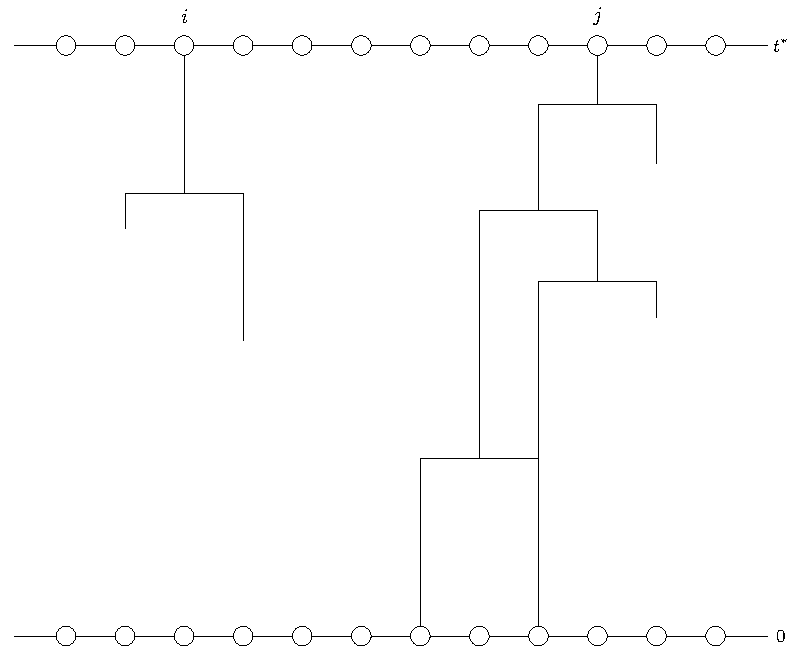
\includegraphics[width = 0.8\textwidth]{Figures/IsingCouplingTime/typical_percolation.pdf}
		\caption[Typical appearance of the update histories for two vertices on the cycle]{A section of the space-time slab $V \times [0, t^*]$ along with a typical appearance of the update histories for two vertices on the cycle. Time runs vertically from bottom to top, and the vertices are represented by circles, laid out horizontally. If there is a path in the update history of $v$ between points $(u, t)$ and $(v, t^*)$, then the spin of $v$ at time $t^*$ depends on the spin of $u$ at time $t$. In this example, since there is no path from vertex $(i, t^*)$ to time $0$, the final spin at $i$ does not depend on the initial configuration whereas the final spin at $j$ does.}
		\label{fig:typical percolation}
	\end{figure}

	\subsubsection{The update sequence}
	Recalling our random mapping representation from Section \ref{sec:the coupling time}, we can encode an update of our coupled process with the tuple $(\mathcal{V}, U, S)$, where $S$ is the time of the update, $\mathcal{V}$ is the vertex that is updated, and $U$ is the value of the uniform random variable that tells us whether $\mathcal{V}$ is a plus or minus according to \eqref{eq:plusorminusrules}. The \emph{update sequence} along an interval $(t_0, t_1]$ is the set of these tuples with $t_0 < S \leq t_1$, ordered by $S$ decreasing from $t_1$. 

	Let $(Y_t)_{t \geq 0}$ be a copy of the continuous-time heat-bath Glauber dynamics starting in some state $Y_0 \in \Omega$. So $Y_t = \mathscr{T}_t$ if $Y_0 = (1, 1, \dots, 1)$ and $Y_t = \mathscr{B}_t$ if $Y_0 = (-1, -1, \dots, -1)$. Given the state of $Y$ at time $t_0$, $Y_{t_0}$, the update sequence along $(t_0, t_1]$ contains all the information we need to contruct $Y_{t_1}$. In particular, given the update sequence along the interval $(0, t_1]$, $Y_{t_1}$ is a deterministic function of $Y_0$.

	\subsubsection{The update support function}
	\label{sec: definition update support function}
	Given the update sequence along the interval $(t_1, t_2]$, the \emph{update support function}, $\mathscr{F}(A, t_1, t_2)$, is the minimal set of vertices whose spins at time $t_1$ determine the spins of the vertices in $A$ at time $t_2$. That is, $i \in \mathscr{F}(A, t_1, t_2)$ if and only if there exist states $Y_{t_1}, Y_{t_1}' \in \{-1, +1\}^{V}$ that differ only at $i$ and such that when we construct $Y_{t_2}$ and $Y_{t_2}'$ using the update sequence, $Y_{t_2} \neq Y_{t_2}'$.

	In particular, if $\mathscr{F}(i, 0, t) = \emptyset$ then the spin at vertex $i$ at time $t$ does not depend on the initial state and so for our coupled chains, $\mathscr{B}_t[i] = \mathscr{T}_t[i]$.
	% It follows that
	% \begin{equation}
	% 	\prob \left[ Y_t[v] \neq Y_t'[v] \right] \leq \prob \left[ \mathscr{F}(v, 0, t) \neq \emptyset \right].
	% 	\label{eq:boundXneqY}
	% \end{equation}
	As a consequence of the monotonicity of our coupling, we can make the stronger statement that $\mathscr{T}_t[i] = \mathscr{B}_t[i]$ if and only if $\mathscr{F}(i, 0, t) = \emptyset$ which of course means that
	\begin{equation}
	\label{eq:prob equality of coupling and empty support}
		\prob[\mathscr{T}_t[i] \neq \mathscr{B}_t[i]] = \prob[\mathscr{F}(i, 0, t) \neq \emptyset].
	\end{equation}

	For ease of notation, we will often use the shorthand
	\begin{equation}
		\mathcal{H}_i(t) := \mathscr{F}(i, t, t^*)
	\end{equation}
	where $t^*$ is some target time that should be clear from context. We call this the \emph{update support} of vertex $i$ at time $t$. Tracing $\mathcal{H}_i(t)$ backwards in time from $t^*$ produces a subgraph of $\Omega \times [0, t^*]$ which we write as $\mathcal{H}_i$ and which we call the \emph{update history} of vertex $i$. To be slightly more precise, to produce $\mathcal{H}_i$ we connect $(j,t)$ to $(j,t')$ if $j \in \mathcal{H}_i(t)$ and there are no updates of $j$ along $(t', t]$ and we connect $(j,t)$ to $(j',t)$ if there was an update at $(j, t)$, $j \in \mathcal{H}_i(t)$, $j' \notin \mathcal{H}_i(t)$, and $j' \in \mathcal{H}_i(t+\epsilon)$ for any sufficiently small $\epsilon > 0$.

	Similarly, we also use 
	\begin{equation}
		\hist_A(t) := \mathscr{F}(A, t, t^*)
	\end{equation}
	for the update history of a vertex set $A$ at time $t$ and $\hist_A$ for the update history of vertex set $A$. Note that
	\begin{equation}
		\hist_A(t) = \bigcup_{i \in A} \hist_i(t)
	\end{equation}
	and 
	\begin{equation}
		\hist_A = \bigcup_{i \in A} \hist_i.
	\end{equation}

	% ALSO DEFINE UPDATE SUPPORT
	
	\subsubsection{The update function}
	\label{sec: definition update function}
	It is usually non-trivial to construct the update support function from the update sequence. So in order to give some intuition to the definitions above, we describe another function which contains the update support and which is simple to construct. We define the \emph{update function}, $\mathscr{F}_\mathrm{UPD}(A, t_1, t_2)$, to be the set of all vertices that $A$ can `reach' through the update function. That is, $i \in \mathscr{F}_\mathrm{UPD}(A, t_1, t_2)$ if and only if there exists a subsequence of the updates, $(\mathcal{V}_k, U_k, S_k)$, such that $t_1 < S_1 < S_2, \dots, \leq S_m$ and $i, \mathcal{V}_1, \mathcal{V}_2, \dots, \mathcal{V}_m$ is a path connecting $i$ to some vertex $\mathcal{V}_m \in A$. 

	Just as we traced the update support backwards through time to create the update history, we can also trace $\mathscr{F}_\mathrm{UPD}(i, t, t^*)$ backwards through time to create the analogous \emph{update trace}, $\mathcal{G}_i$. It is clear that $\mathscr{F}(A, t_1, t_2) \subseteq \mathscr{F}_\mathrm{UPD}(A, t_1, t_2)$ since a vertex $i$ can only affect the spins of $A$ if there is a path of updates connecting it to $A$. Likewise we also have that $\mathcal{G}_i \subseteq \hist_i$.
	
	Consider how we can construct the update trace of a vertex $i$ from some target time $t^*$. We have at our disposal the update sequence along $(0, t^*]$ which is placed in order of decreasing time. If vertex $i$ does not appear in the update sequence then we create a temporal edge between $(i, t^*)$ and $(i, 0)$ and our update history is complete. Otherwise, we create a temporal edge between $(i, t^*)$ and $(i, t_i)$ where $t_i$ is the last time vertex $i$ was updated. At this point we add spatial edges from $(i, t_i)$ to $(j, t_i)$ for each $j\sim i$. Then, we iterate this process for $i$ and each of its neighbours starting at time $t_i$ until every edge has reached time $0$. In Figure \ref{fig:example trace construction} we have followed this procedure to show an example update trace for a single vertex on the cycle. 

	\begin{figure}
		\centering
		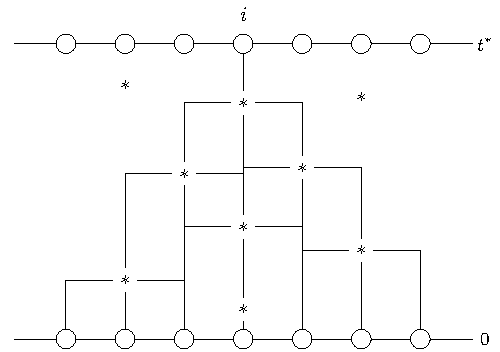
\includegraphics[width = 0.8\textwidth]{Figures/IsingCouplingTime/example_update_trace_construction.pdf}
		\caption[The update trace of i]{The update trace of $i$. Each update $(\mathcal{V}, U, t)$ in the update sequence is represented by a $*$ at $(\mathcal{V}, t)$.}
		\label{fig:example trace construction}
	\end{figure}

	We turn now to discussing how the update history differs from the update trace. We first note that an update to vertex $i$ removes it from the update support as we move backwards in time. This is because the updated spin at $i$ is a function only of its neighbours \eqref{eq:plusorminusrules}. The second difference which we will now spend some time discussing is that it is possible for updates to occur that do not depend on neighbouring spins. These updates therefore cause temporal edges leading up to them to terminate without branching out to the neighbouring vertices. These type of updates are called \emph{oblivious updates}. (These are not the only differences between the update history and the update trace; there are other ways in which vertices can be removed from the update support. See Figure \ref{fig:nonoblivious shrink} for an example).

	% \begin{figure}
	% 	\centering
	% 	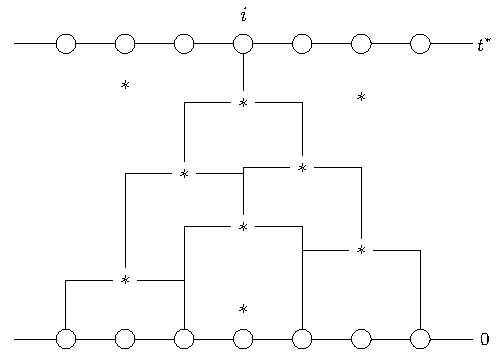
\includegraphics[width = 0.8\textwidth]{Figures/IsingCouplingTime/example_percolation_construction.pdf}
	% 	\caption[A naive construction of the update history of i]{A naive construction of the update history of $i$. Each update $(\mathcal{V}, U, t)$ in the update sequence is represented by a $*$ at $(\mathcal{V}, t)$.}
	% 	\label{fig:example percolation construction}
	% \end{figure}

	

	\subsubsection{Oblivious updates}
	\label{sec:oblivious updates}

	Roughly speaking, an update to a vertex is oblivious if we do not need to know the configuration of its neighbours to determine the spin of that vertex. More precisely, an update, $(\mathcal{V}, U, t)$, is oblivious if and only if
	%for any $\sigma_1, \sigma_2 \in \Omega$, $\sigma_1' = f(\sigma_1, \mathcal{V}, U)$ and $\sigma_2' = f(\sigma_2, \mathcal{V}, U)$ are such that
	% \begin{equation}
	% 	\sigma_1'[\mathcal{V}] = \sigma_2'[\mathcal{V}].
	% \end{equation}
	\begin{equation}
		f(\sigma, \mathcal{V}, U)[\mathcal{V}] = f(\sigma', \mathcal{V}, U)[\mathcal{V}]
	\end{equation}
	for all $\sigma, \sigma' \in \Omega$, where $f$ is as defined in \eqref{eq:plusorminusrules}.

	Consider how these updates occur under our random mapping representation. Let $\Delta_i$ denote the degree of a vertex $i$. Recalling \eqref{eq:define p_i},
	\begin{equation}
		\frac{\euler^{-\beta \Delta_i}}{\euler^{\beta \Delta_i} + \euler^{-\beta \Delta_i}} \leq p_i(\sigma) \leq \frac{\euler^{\beta \Delta_i}}{\euler^{\beta \Delta_i} + \euler^{-\beta \Delta_i}},
	\end{equation}
	with equality holding for the lower and upper limits when the neighbours have spins all minus and all plus respectively. So for a particular update $(\mathcal{V}, U, t)$, if $U \leq \frac{\euler^{-\beta \Delta_\mathcal{V}}}{\euler^{\beta \Delta_\mathcal{V}} + \euler^{-\beta \Delta_\mathcal{V}}}$ then $\mathcal{V}$ is updated to a plus regardless of the configuration of its neighbours. Hence $(\mathcal{V}, U, t)$ is an oblivious update. Similarly, if $U > \frac{\euler^{\beta \Delta_\mathcal{V}}}{\euler^{\beta \Delta_\mathcal{V}} + \euler^{-\beta \Delta_\mathcal{V}}}$ then $\mathcal{V}$ is updated to a minus regardless of the configuration of its neighbours and hence $(\mathcal{V}, U, t)$ is an oblivious update. It is easy to see that these are the only types of oblivious updates.
	
	Given an update at vertex $i$, the probability that this update is oblivious is
	\begin{align}
		\theta_i &= 1 - \left(\frac{\euler^{\beta \Delta_i}}{\euler^{\beta \Delta_i} + \euler^{-\beta \Delta_i}} - \frac{\euler^{-\beta \Delta_i}}{\euler^{\beta \Delta_i} + \euler^{-\beta \Delta_i}}\right)\\
			&= 1 - \tanh(\beta \Delta_i).
	\end{align}
	If $G$ is a $\Delta$-regular graph (as will be the case in the following chapters) then we can drop the subscript and write $\theta = 1 - \tanh(\beta \Delta)$ for the probability of an oblivious update at each vertex.

	As noted earlier, oblivious updates cause temporal edges leading to them in the update history to terminate. If $j \in \mathcal{H}_i(t)$, then an oblivious update $(j, u, t)$ removes $j$ from $\mathcal{H}_i(t)$ without adding any of its neighbours. In Figure \ref{fig:example percolation construction oblivious} we construct the update history from a single vertex $i$ using the same update sequence as in Figure \ref{fig:example trace construction} but instead of representing each update with just a $*$, we give a little more information in the following way. Note that on the cycle, the function defined in \eqref{eq:plusorminusrules} can be rewritten as
	\begin{equation}
		\sigma'[i] = 
		\begin{cases}
			1 & U \leq \theta/2,\\
			\sigma[i-1] \vee \sigma[i+1] & \theta/2 < U \leq 1/2,\\
			\sigma[i-1] \wedge \sigma[i+1] & 1/2 < U \leq 1 - \theta/2,\\
			-1	& U > \theta/2.
		\end{cases}
	\end{equation}
	We can therefore represent each update $(\mathcal{V}, U, t)$ in the update sequence by placing at $(\mathcal{V}, t)$ one of the symbols $+$, $\vee$, $\wedge$, or $-$ choosen according to $U$. We then trace back from time $t^*$, branching to either side when we encounter a $\vee$ or $\wedge$, and terminating whenever we encounter a $+$ or $-$.

	\begin{figure}
		\centering
		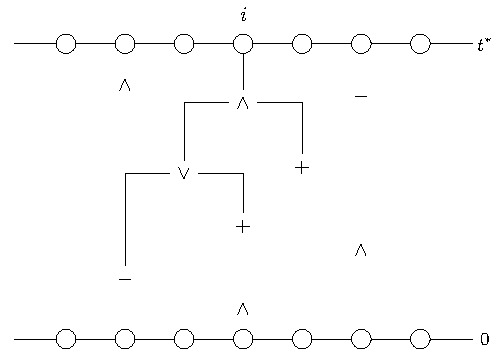
\includegraphics[width = 0.8\textwidth]{Figures/IsingCouplingTime/example_percolation_construction_oblivious.pdf}
		\caption[The update sequence for a section of the cycle and the corresponding update history from vertex i]{The update sequence for a section of the cycle and the corresponding update history from vertex $i$. For this particular update sequence, $i$ takes a final spin of $+1$ regardless of the initial configuration.}
		\label{fig:example percolation construction oblivious}
	\end{figure}

	
	It is worth remarking that oblivious updates are not necessarily the only updates that can shrink the size of the update history of $i$. In Figure \ref{fig:nonoblivious shrink} we use an example from \cite{Lubetzky2016-wd} that shows the update support collapsing down to a single vertex from a non-oblivious update. However, for our analysis, oblivious updates will be the only such updates we will be concerned with. Indeed, in Chapter \ref{Ch:1D} we will use a different coupling so that these are the only updates that shrink the size of the update history, and in Chapter \ref{Ch:GeneralResults} we will use an alternative construction that bounds the true update history, in which all updates are either oblivious or branch out to all $\Delta$ neighbours.

	\begin{figure}
		\centering
		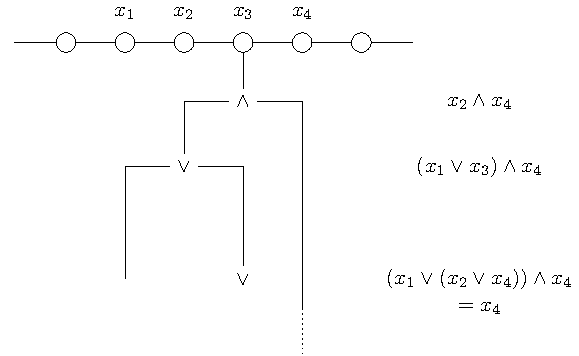
\includegraphics[width = 0.8\textwidth]{Figures/IsingCouplingTime/nonoblivious_shrink.pdf}
		\caption[A non-oblivious update that shrinks the size of the update history]{[Example taken from \cite{Lubetzky2016-wd}]. A non-oblivious update that shrinks the size of the update history. On the right is written the final spin of $x_3$ as a function of the configuration at that time. The update $x_3 \mapsto x_2 \vee x_4$ causes the entire function to collapse to $x_4$, and so removes $x_1$ and $x_3$ from the update history.}
		\label{fig:nonoblivious shrink}
	\end{figure}
	

